\documentclass[]{article}
\usepackage{lmodern}
\usepackage{amssymb,amsmath}
\usepackage{ifxetex,ifluatex}
\usepackage{fixltx2e} % provides \textsubscript
\ifnum 0\ifxetex 1\fi\ifluatex 1\fi=0 % if pdftex
  \usepackage[T1]{fontenc}
  \usepackage[utf8]{inputenc}
\else % if luatex or xelatex
  \ifxetex
    \usepackage{mathspec}
  \else
    \usepackage{fontspec}
  \fi
  \defaultfontfeatures{Ligatures=TeX,Scale=MatchLowercase}
\fi
% use upquote if available, for straight quotes in verbatim environments
\IfFileExists{upquote.sty}{\usepackage{upquote}}{}
% use microtype if available
\IfFileExists{microtype.sty}{%
\usepackage[]{microtype}
\UseMicrotypeSet[protrusion]{basicmath} % disable protrusion for tt fonts
}{}
\PassOptionsToPackage{hyphens}{url} % url is loaded by hyperref
\usepackage[unicode=true]{hyperref}
\hypersetup{
            pdfborder={0 0 0},
            breaklinks=true}
\urlstyle{same}  % don't use monospace font for urls
\usepackage{graphicx,grffile}
\makeatletter
\def\maxwidth{\ifdim\Gin@nat@width>\linewidth\linewidth\else\Gin@nat@width\fi}
\def\maxheight{\ifdim\Gin@nat@height>\textheight\textheight\else\Gin@nat@height\fi}
\makeatother
% Scale images if necessary, so that they will not overflow the page
% margins by default, and it is still possible to overwrite the defaults
% using explicit options in \includegraphics[width, height, ...]{}
\setkeys{Gin}{width=\maxwidth,height=\maxheight,keepaspectratio}
\IfFileExists{parskip.sty}{%
\usepackage{parskip}
}{% else
\setlength{\parindent}{0pt}
\setlength{\parskip}{6pt plus 2pt minus 1pt}
}
\setlength{\emergencystretch}{3em}  % prevent overfull lines
\providecommand{\tightlist}{%
  \setlength{\itemsep}{0pt}\setlength{\parskip}{0pt}}
\setcounter{secnumdepth}{0}
% Redefines (sub)paragraphs to behave more like sections
\ifx\paragraph\undefined\else
\let\oldparagraph\paragraph
\renewcommand{\paragraph}[1]{\oldparagraph{#1}\mbox{}}
\fi
\ifx\subparagraph\undefined\else
\let\oldsubparagraph\subparagraph
\renewcommand{\subparagraph}[1]{\oldsubparagraph{#1}\mbox{}}
\fi

% set default figure placement to htbp
\makeatletter
\def\fps@figure{htbp}
\makeatother


\date{}

\begin{document}

\begin{quote}
La percolation \textsuperscript{1} désigne le passage d'un fluide à
travers un solide poreux. Ce terme fait bien entendu référence au café
produit par le passage de l'eau à travers une poudre de café comprimée,
mais dans un sens plus large peut aussi bien s'appliquer à
l'infiltration des eaux de pluie jusqu'aux nappes phréatiques ou encore
à la propagation des feux de forêt par contact entre les feuillages des
arbres voisins.

L'étude scientifique des modèles de percolation s'est développée à
partir du milieu du XXe siècle et touche aujourd'hui de nombreuses
disciplines, allant des mathématiques à l'économie en passant par la
physique et la géologie.
\end{quote}

\section{Choix d'un modèle}\label{choix-dun-moduxe8le}

\begin{quote}
Nous allons aborder certains phénomènes propres à la percolation par
l'intermédiaire d'un modèle très simple : une grille carrée \emph{n n},
chaque case pouvant être ouverte (avec une probabilité \emph{p}) ou
fermée (avec une probabilité 1 \emph{p}). La question à laquelle nous
allons essayer de répondre est la suivante : est-il possible de joindre
le haut et le bas de la grille par une succession de cases ouvertes
adjacentes ?

Figure 1 -- \emph{deux exemples de grilles} 10 10 \emph{; la percolation
n'est possible que dans le second cas (les cases ouvertes sont les cases
blanches).}

On conçoit aisément que la réussite ou non de la percolation dépend
beaucoup de \emph{p} : plus celle-ci est grande, plus les chances de
réussite sont importantes. Nous auront l'occasion d'observer l'existence
pour de grandes valeurs de \emph{n} d'un seuil critique
\emph{p}\textsubscript{0} au delà duquel la percolation a toutes les
chances de réussir et en deçà duquel la percolation échoue presque à
chaque fois.
\end{quote}

\section{Création et visualisation de la
grille}\label{cruxe9ation-et-visualisation-de-la-grille}

\begin{quote}
Les deux modules essentiels dont nous aurons besoin sont les modules
numpy (manipulation de tableaux bi-dimensionnels) et mathplotlib.pyplot
(graphisme), qu'il convient d'importer :

Nous aurons aussi besoin de la fonction rand du module numpy.random
(fonction qui retourne un nombre pseudo- aléatoire de l'intervalle
{[}0\emph{,} 1{[}) et accessoirement de la fonction ListedColormap du
module matplotlib.colors (pour choisir l'échelle chromatique à utiliser
pour la représentation graphique). Ces deux fonctions seront importées
directement, puisque nous n'aurons pas besoin des modules entiers :

La grille de percolation sera représentée par le type np.array. La
fonction np.zeros((n, p)) renvoie un tableau de \emph{n} lignes et
\emph{p} colonnes contenant dans chacune de ses cases le nombre flottant
0.0. Une fois un tableau tab créé, la case d'indice (\emph{i, j}) est
référencée indifféremment par tab{[}i{]}{[}j{]} ou par tab{[}i, j{]} et
peut être lue et modifiée (comme d'habitude, les indices débutent à 0).
Enfin, on notera que si tab est un tableau, l'attribut tab.shape
retourne le couple (\emph{n, p}) de ses dimensions verticale et
horizontale (le nombre de lignes et de colonnes, tab étant vu comme une
matrice).

1. du latin \emph{percolare} : couler à travers.

Dans la suite de ce document, on représentera une grille de percolation
par un tableau \emph{n n}, les cases fermées contenant le nombre
flottant 0.0 et les cases ouvertes le nombre flottant 1.0.

Question 1. Définir une fonction creation\_grille(p, n) à deux
paramètres : un nombre réel \emph{p} (qu'on supposera dans l'intervalle
{[}0\emph{,} 1{[}) et un entier naturel \emph{n}, qui renvoie un tableau
\emph{n n} dans lequel chaque case sera ouverte avec la probabilité
\emph{p} et fermée sinon.

Pour visualiser simplement la grille, nous allons utiliser la fonction
plt.matshow : appliquée à un tableau, celle-ci présente ce dernier sous
forme de cases colorées en fonction de leur valeur \textsuperscript{2}.
Les couleurs sont choisies en fonction d'une échelle chromatique que
vous pouvez visualiser à l'aide de la fonction plt.colorbar(). Celle
utilisée par défaut va du bleu au rouge ; puisque nos grilles ne
contiennent pour l'instant que les valeurs 0 ou 1, les cases fermées
apparaîtrons en bleu, et les cases ouvertes, en rouge.

Changer l'échelle chromatique

L'argument par défaut cmap de la fonction plt.matshow permet de modifier
l'échelle chromatique utilisée. La fonction ListedColormap va nous
permettre de créer l'échelle de notre choix. Puisque nous n'aurons que
trois états possibles (une case pleine représentée par la valeur 0.0),
une case vide représentée par la valeur 1.0 et plus tard une case
remplie d'eau représentée par la valeur 0.5) une échelle à trois
couleurs suffit. Vous pouvez utiliser celle-ci :

ou celle de votre choix, dans la limite du bon goût.

(Vous trouverez la liste des couleurs prédéfinies à l'adresse
http://www.python−simple.com/img/img36.png)
\end{quote}

\section{Percolation}\label{percolation}

\begin{quote}

\includegraphics[width=0.82943in,height=0.47396in]{media/image1.png}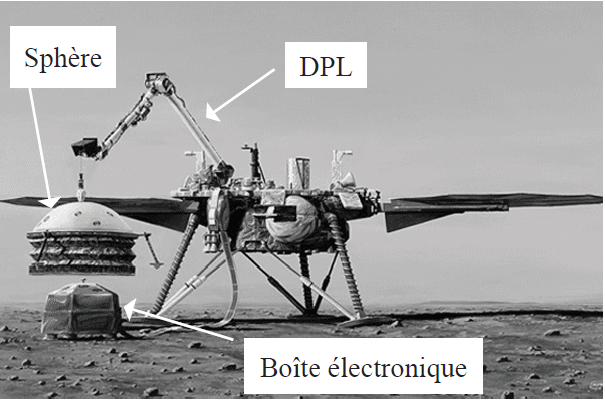
\includegraphics{media/image2.png}Une
fois la grille crée, les cases ouvertes de la première ligne sont
remplies par un fluide, ce qui sera représenté par la valeur 0.5 dans
les cases correspondantes. Le fluide pourra ensuite être diffusé à
chacune des cases ouvertes voisines d'une case contenant déjà le fluide
jusqu'à remplir toutes les cases ouvertes possibles.

Figure 2 -- \emph{les deux grilles de la figure 1, une fois le processus
de percolation terminé (le fluide est représenté par des hachures).}

Question 2. Écrire une fonction percolation qui prend en argument une
grille et qui remplit de fluide celle-ci, en appliquant l'algorithme
exposé ci-dessous.
\end{quote}

\begin{enumerate}
\def\labelenumi{(\roman{enumi})}
\item
  Créer une liste contenant initialement les coordonnées des cases
  ouvertes de la première ligne de la grille et remplir ces cases de
  liquide.
\item
  Puis, tant que cette liste n'est pas vide, e ffectuer les opérations
  suivantes :
\end{enumerate}

\begin{quote}
--extraire de cette liste les coordonnées d'une case quelconque ;

--ajouter à la liste les coordonnées des cases voisines qui sont encore
vides, et les remplir de liquide.

L'algorithme se termine quand la liste est vide.

Rédiger un script vous permettant de visualiser une grille avant et
après remplissage, et faire l'expérience avec quelques valeurs de
\emph{p} pour une grille de taille raisonnable (commencer avec \emph{n}
= 64 pour vérifier visuellement que votre algorithme est correct, puis
augmenter la taille de la grille, par exemple avec \emph{n} = 512).

On dit que la percolation est réussie lorsqu'à la fin du processus au
moins une des cases de la dernière ligne est remplie du fluide.

Question 3. Écrire une fonction teste\_percolation qui prend en argument
un réel \emph{p} {[}0\emph{,} 1{[} et un entier \emph{n}
N\textsuperscript{∗}, crée une grille, effectue la percolation et
retourne :
\end{quote}

\begin{itemize}
\item
  True lorsque la percolation est réussie, c'est-à-dire lorsque le bas
  de la grille est atteint par le fluide ;
\item
  False dans le cas contraire.
\end{itemize}

\section{Seuil critique}\label{seuil-critique}

\begin{quote}
Nous allons désormais travailler avec des grilles de taille 128 128
\textsuperscript{3}. Faire quelques essais de percolation avec
différentes valeurs de \emph{p}. Vous observerez assez vite qu'il semble
exister un seuil \emph{p}\textsubscript{0} en deçà duquel la percolation
échoue presque à chaque fois, et au delà duquel celle-ci réussit presque
à chaque fois. Plus précisément, il est possible de montrer que pour une
grille de taille infinie, il existe un seuil critique
\emph{p}\textsubscript{0} en deçà duquel la percolation échoue toujours,
et au delà duquel la percolation réussit toujours. Bien évidemment, plus
la grille est grande, plus le comportement de la percolation tend à se
rapprocher du cas de la grille théorique infinie.

Question 4. Notons P(\emph{p}) la probabilité pour le fluide de
traverser la grille.
\end{quote}

\begin{enumerate}
\def\labelenumi{\alph{enumi})}
\item
  Proposer une démarche expérimentale simple pour estimer cette quantité
  en fonction de \emph{p}, et rédiger la fonction
\end{enumerate}

\begin{quote}
proba correspondante.

P(\emph{p})
\end{quote}

1

\begin{quote}
\emph{p}

\emph{p}0 1

Figure 3 -- \emph{L'allure théorique du graphe de la fonction} P\emph{.}
\end{quote}

\begin{enumerate}
\def\labelenumi{\alph{enumi})}
\item
  En utilisant une recherche dichotomique, chercher à estimer le plus
  précisément possible la valeur numérique du seuil
  \emph{p}\textsubscript{0}.
\end{enumerate}

\section{Propriétés
macroscopiques}\label{propriuxe9tuxe9s-macroscopiques}

\begin{quote}
A l'instar de la thermodynamique, on peut décrire le comportement d'un
système lors d'une transition de phase en introduisant des propriétés
macroscopiques. Dans le cas de la percolation, on peut par exemple
définir la densité moyenne \emph{d}(\emph{p}) de cases ouvertes
atteintes par le fluide.

Question 5.
\end{quote}

\begin{enumerate}
\def\labelenumi{\alph{enumi})}
\item
  Définir une fonction densite qui prend en argument une grille dans
  laquelle la percolation a eu lieu et qui retourne la valeur de sa
  densité.
\item
  À l'aide d'un nombre raisonnable d'échantillons, définir alors la
  fonction d qui à une probabilité \emph{p} ∈ {[}0\emph{,} 1{[} associe
  la densité moyenne de la percolation dans une grille 128 × 128.
\item
  Tracer le graphe de \emph{d}(\emph{p}) pour \emph{p} ∈ {[}0\emph{,}
  1{[}.
\end{enumerate}

\section{Et pour les plus rapides}\label{et-pour-les-plus-rapides}

\begin{quote}
Recommencez toute cette étude, mais cette fois-ci avec une grille
hexagonale. Il est possible de prouver que pour une grille hexagonale
carrée le seuil critique \emph{p}\textsubscript{0} est exactement égal à
\emph{p}\textsubscript{0} = 1\emph{/}2 ; le vérifier expérimentalement
et chercher à le démontrer (en utilisant un argument de symétrie).
\end{quote}

\end{document}
